\documentclass[10pt]{book}

%These tell TeX which packages to use.
\usepackage{array,epsfig}
\usepackage{amsmath}
\usepackage{amsfonts}
\usepackage{amssymb}
\usepackage{amsxtra}
\usepackage{amsthm}
\usepackage{mathrsfs}
\usepackage{color}
\usepackage{enumitem}
%\usepackage{mdframed}
\usepackage[most]{tcolorbox}
\usepackage{pgfplots}
\pgfplotsset{compat=1.6}

\pgfplotsset{soldot/.style={color=black,only marks,mark=*}} \pgfplotsset{holdot/.style={color=black,fill=white,only marks,mark=*}}

%Here I define some theorem styles and shortcut commands for symbols I use often
\theoremstyle{definition}
\newtheorem{defn}{Definition}
\newtheorem{thm}{Theorem}
\newtheorem{cor}{Corollary}
\newtheorem*{rmk}{Remark}
\newtheorem{lem}{Lemma}
\newtheorem*{joke}{Joke}
\newtheorem{ex}{Example}
\newtheorem*{soln}{Solution}
\newtheorem{prop}{Proposition}

\newcommand{\lra}{\longrightarrow}
\newcommand{\ra}{\rightarrow}
\newcommand{\surj}{\twoheadrightarrow}
\newcommand{\graph}{\mathrm{graph}}
\newcommand{\bb}[1]{\mathbb{#1}}
\newcommand{\Z}{\bb{Z}}
\newcommand{\Q}{\bb{Q}}
\newcommand{\R}{\bb{R}}
\newcommand{\C}{\bb{C}}
\newcommand{\N}{\bb{N}}
\newcommand{\M}{\mathbf{M}}
\newcommand{\m}{\mathbf{m}}
\newcommand{\MM}{\mathscr{M}}
\newcommand{\HH}{\mathscr{H}}
\newcommand{\Om}{\Omega}
\newcommand{\Ho}{\in\HH(\Om)}
\newcommand{\bd}{\partial}
\newcommand{\del}{\partial}
\newcommand{\bardel}{\overline\partial}
\newcommand{\textdf}[1]{\textbf{\textsf{#1}}\index{#1}}
\newcommand{\img}{\mathrm{img}}
\newcommand{\ip}[2]{\left\langle{#1},{#2}\right\rangle}
\newcommand{\inter}[1]{\mathrm{int}{#1}}
\newcommand{\exter}[1]{\mathrm{ext}{#1}}
\newcommand{\cl}[1]{\mathrm{cl}{#1}}
\newcommand{\ds}{\displaystyle}
\newcommand{\vol}{\mathrm{vol}}
\newcommand{\cnt}{\mathrm{ct}}
\newcommand{\osc}{\mathrm{osc}}
\newcommand{\LL}{\mathbf{L}}
\newcommand{\UU}{\mathbf{U}}
\newcommand{\support}{\mathrm{support}}
\newcommand{\AND}{\;\wedge\;}
\newcommand{\OR}{\;\vee\;}
\newcommand{\Oset}{\varnothing}
\newcommand{\st}{\ni}
\newcommand{\wh}{\widehat}
%Pagination stuff.
\setlength{\topmargin}{-0.75in}
\setlength{\oddsidemargin}{0in}
\setlength{\evensidemargin}{0in}
\setlength{\textheight}{9.in}
\setlength{\textwidth}{6.5in}
\pagestyle{empty}
\begin{document}
\begin{flushleft}
Name:\underline{\hspace{13cm}}Date:\underline{\hspace{2cm}}
\end{flushleft}
\begin{center}
{\Large Math 1041-007 \hspace{0.5cm} Section 2.5: Continuity}
\end{center}
%\vspace{0.2 cm}

\begin{tcolorbox}
\subsection*{Definition of Continuity}
A function $f$ is \textbf{continuous at a number a} if 
\[
\lim_{x\rightarrow a}f(x)=f(a).
\]
This implies three things:
\begin{itemize}
    \item[(i)] $f(a)$ is defined
    \item[(ii)] $\displaystyle\lim_{x\rightarrow a}f(x)$ exists.
    \item[(iii)]$\displaystyle\lim_{x\rightarrow a}f(x)=f(a)$
\end{itemize}
If one of these \underline{does not happen} then we say that $f(x)$ is discontinuous at ``$a$''.
\end{tcolorbox}
\subsection*{Intro. Example: Using a graph}
The figure below shows the graph of a function $f(x)$. At which numbers is $f$ discontinuous? Explain why? there is a discontinuity!
\begin{figure}[h!]
    \centering
    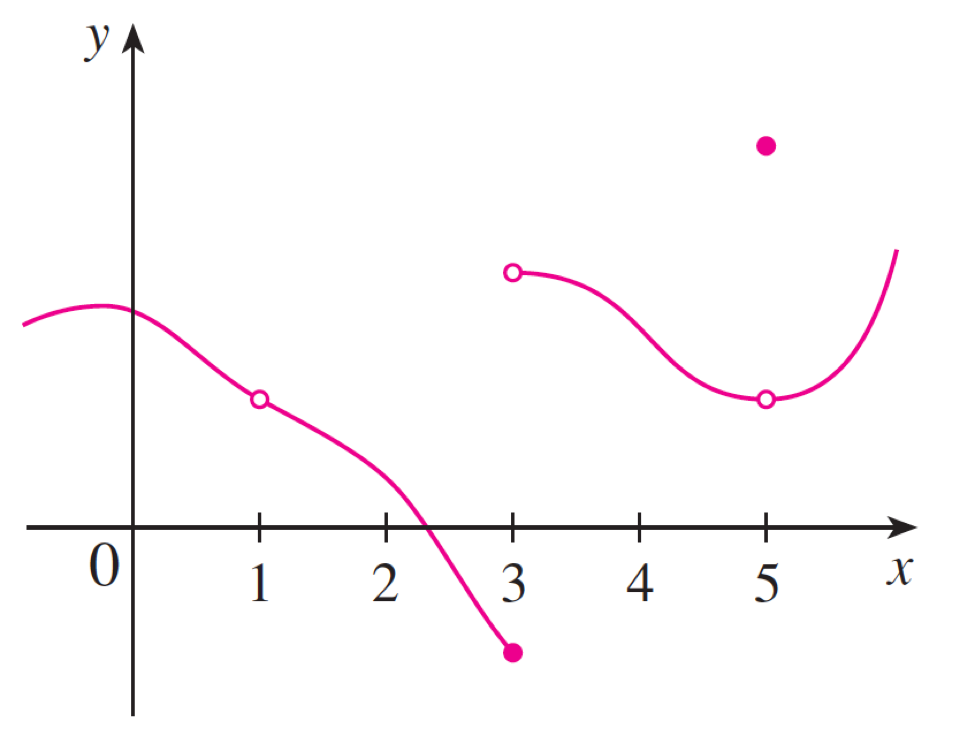
\includegraphics[scale=0.5]{fig1.png}
\end{figure}
\clearpage
\subsection*{Example 1: Detecting \& Classifying Discontinuities from Formulas}
Where are each of the following functions discontinuous??
\begin{itemize}
    \item[(a)] $\displaystyle f(x)=\frac{x^2-x-2}{x-2}$\vspace{4cm}
    \item[(b)] $\displaystyle f(x) = \begin{cases}
      \displaystyle\frac{1}{x^2} & \text{if }x \neq 0 \\[4pt]
      1 & \text{if }x = 0
    \end{cases}$\vspace{4cm}
    \item[(c)]$f(x)\begin{cases}\displaystyle\frac{x^2-x-2}{x-2} & \text{if } x\neq 2\\[4pt] 1 & \text{if }x=2\end{cases}$\vspace{4cm}
    \item[(d)]$f(x)=\begin{cases}1 & \text{if }x<0\\
    2 & \text{if} x\geq 0\end{cases}$
\end{itemize}
\raggedbottom
\clearpage
\begin{tcolorbox}
\subsection*{One-sided Continuity}
\begin{itemize}
    \item A function is \textbf{continuous from the right at a number ``$a$''} if $\displaystyle\lim_{x\rightarrow a^+}f(x)=f(a)$
    In other words approaching ``$a$'' from the right equals the endpoint
    \item A function is \textbf{continuous from the left at a number ``$a$''} if $\displaystyle\lim_{x\rightarrow a^-}f(x)=f(a)$
    In other words approaching ``$a$'' from the left equals the endpoint
\end{itemize}
\subsection*{Definition: Continuous on an interval}
A function is continuous on an interval if it is continuous at every number \underline{in} the interval. \\ \\
Pencil analogy: if the curve between two endpoints on an interval can be drawn without lifting your pencil, then you have continuity on the interval.
\end{tcolorbox}
\subsection*{Example 2: Describe the continuity}
Given the function $f(x)=1-\sqrt{1-x^2}$
\begin{itemize}
    \item State the domain of this function.
    \item Where is this function continuous?
    \item Make a rough sketch of this function
\end{itemize}
\raggedbottom
\clearpage
\begin{tcolorbox}
\subsection*{Theorems and More Theorems}
\underline{\textbf{Theorem I}} If $f,g$ are continuous at ``$a$'' and $c$ is a constant, then $f+g$, $f-g$, $fg$, and $cf$ are also continuous. We also have $\displaystyle \frac{f}{g}$ is continuous \underline{if} $g(a)\neq 0$.\\ \\
\underline{\textbf{Theorem II}} A polynomial is continuous everywhere, $(-\infty,\infty)$.\\ \\
\underline{\textbf{Theorem III}} The following types of functions are continuous at every number \textbf{inside their domains}: polynomials, rational functions, root functions, trig functions, inverse trig, exponential, logarithmic functions.
\end{tcolorbox}
\subsection*{Example 3: Using Continuity}
\begin{itemize}
    \item[(a)] Use continuity to find $\displaystyle \lim_{x\rightarrow 4}\frac{1+\sqrt{x-1}}{\sqrt{5+x}}$ (Hint: start by finding the domain!)\vspace{3cm}
    \item[(b)] Find $\displaystyle\lim_{x\rightarrow -2}\frac{x^3+2x^2-1}{5-3x}$.\vspace{4cm}
    \item[(c)] Where is $\displaystyle f(x)=\frac{\ln x+\tan^{-1}x}{x^2-1}$ continuous?
    \vspace{4cm}
    \item[(d)] Evaluate $\displaystyle\lim_{x\rightarrow \pi}\frac{\sin x}{2+\cos x}$.
    \end{itemize}
    \raggedbottom
    \clearpage
    \begin{tcolorbox}
    \subsection*{Continuity of Composite Functions}
    \begin{itemize}
        \item (Pass the Limit Inside Rule) If $f$ is continuous at $b$ and $\displaystyle\lim_{x\rightarrow a}g(x)=b$ then
        \[
        \lim_{x\rightarrow a}f(g(x))=f\left(\lim_{x\rightarrow a}g(x)\right)
        \]
        \item (Composition of Continuous IS continuous) If $g$ is continuous at $a$ and $f$ is continuous at $g(a)$, then $f(g(x))$ is continuous at $a$.
    \end{itemize}
    \end{tcolorbox}
    \subsection*{Example 4: Using Composition}
    \begin{itemize}
        \item[(a)] Evaluate $\displaystyle\lim_{x\rightarrow 1}\arcsin\left(\frac{1-\sqrt{x}}{1-x}\right)$ \vspace{4cm}
        \item[(b)] Where is $h(x)=\sin(x^2)$ continuous?\vspace{4cm}
        \item[(c)] Where is $F(x)=\ln(1+\cos x)$ continuous?
    \end{itemize}
    \raggedbottom
    \clearpage
    \begin{tcolorbox}
    \subsection*{Intermediate Value Theorem (IVT)} Given a continuous function $f$ on a closed interval $[a,b]$, and suppose you pick a value $N$ that is between $f(a)$ and $f(b)$. Then $N$ has a corresponding $c$ value in $(a,b)$ such that $f(c)=N$.\\ \\
    Or in other words given a continuous function on a closed interval, then every $y$ in the range has a corresponding $x$ (at least one) in the domain:
    \end{tcolorbox}
    \begin{figure}[h!]
        \centering
        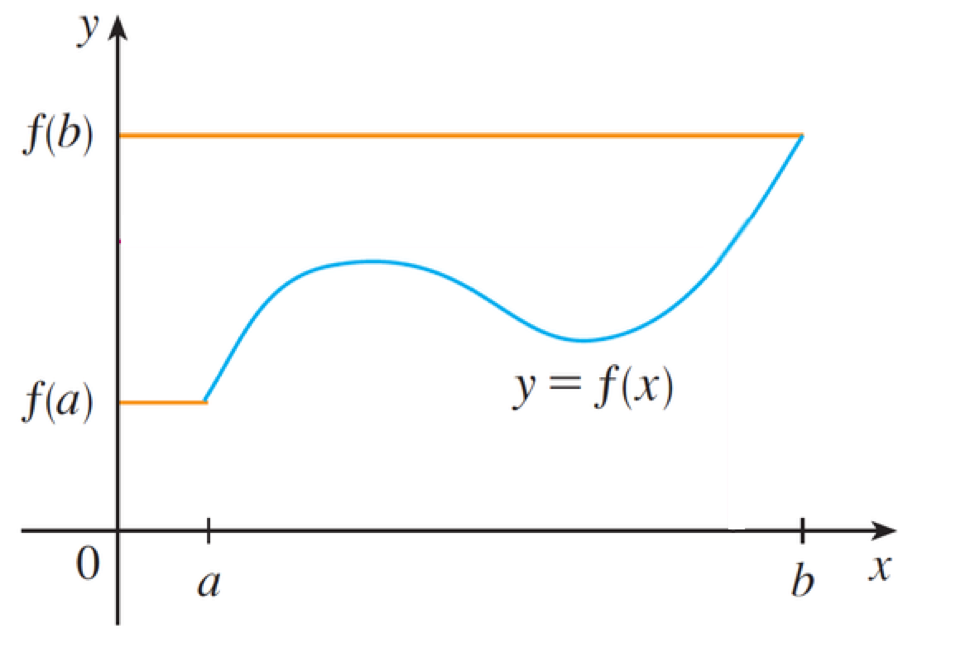
\includegraphics[scale=0.5]{fig2.png}
    \end{figure}
    \subsection*{Example 5: Using IVT}
    Show that there is a root of the equation
    \[
    4x^3-6x^2+3x-2=0
    \]
    between $1$ and $2$.
\end{document}